\documentclass[12pt,english]{article}
\usepackage{geometry}
\geometry{verbose,letterpaper,tmargin=2.54cm,bmargin=2.54cm,lmargin=2.54cm,rmargin=2.54cm}
\usepackage[T1]{fontenc}
\usepackage{lmodern}
\usepackage{amssymb,amsmath}
\usepackage{ifxetex,ifluatex}
\usepackage{natbib}
\bibliographystyle{plainnat}
\usepackage{graphicx}
\usepackage{caption}
\usepackage{subcaption}
\usepackage{brush_style}
\usepackage{setspace}
\usepackage{lineno}
\linenumbers
\title{Persistence of marine populations under climate and fishing}
\author{Emma Fuller, Eleanor Brush, Malin Pinsky}
\date{}

\begin{document}
\maketitle

\begin{spacing}{1.9}
\begin{flushleft}

\section{Abstract}

When the climate changes, the habitat with suitable conditions in which organisms can survive and reproduce moves. 
This change does not occur in isolation but rather appears on a background of other disturbances. 
In order to understand how two disturbances, range shift and harvesting, interact and affect population persistence, we studied an integrodifference model that explicitly included the mechanisms of dispersal and reproduction.  If the viable habitat moves too quickly or harvesting pressure is too great, the population is driven extinct.  We found the rates of harvesting and environmental shift required to allow the population to persist and and studied how these critical parameters depend on the growth rate and dispersal behavior of the population.  We then measured the interaction between the stressors.  The stressors interact nearly additively: we found very low positive synergy at those levels of the stressors that almost drive the population extinct.  Positive synergy suggests that harvesting may aggravate the population's sensitivity to a shifting range. Finally, we introduced two conservation techniques into simulations of the population model -- threshold harvest rules and marine protected areas (MPAs) -- and found that under some circumstances these approaches could mitigate the interaction between the two stressors.  
\hspace{10cm}

\noindent {\bf Keywords:} Climate change, fishing, integrodifference model, synergy, multiple disturbances

\section{Introduction}

There are many stressors that can disturb an ecosystem. Ecologists have quantified the effects of a number of stressors individually \citep{Wilcoveetal1998, Crainetal2008, DarlingCote2008}, but less work has been done to measure the effects of multiple stressors and the interactions between them.  If disturbances interact synergistically, a perturbation that has little effect when it occurs individually may amplify the disturbance caused by a coincident perturbation \citep{Crainetal2008, DarlingCote2008,Nyeetal2013,Gurevitchetal2000}.   In the most extreme (and worrying) cases, synergistic interactions between multiple stressors will drive a population extinct even though it could persist in the face of any single stressor (e.g. \citet{Pelletieretal2006}).  If disturbances interact antagonistically, on the other hand, the effects of multiple stressors may be less than that predicted by the individual effects of the stressors.  Since disturbances rarely occur in isolation, it is important to measure the synergy between  disturbances in order to understand how a system will be affected by their presence and to understand when multiple disturbances will drive a population extinct  \citep{DoakMorris2010, Fordhametal2013, Foltetal1999}.


Climate change and fishing have been identified as the two largest human impacts on the ocean \citep{Halpernetal2008}.  They therefore provide an important case study of how disturbances interact in their effects on biological populations.  Further, understanding these interactions will be crucial to managing populations subjected to both of these disturbances.  Marine fish are already moving in response to climate change \citep{Perryetal2005, HiddinkHoftstede2008, Rijnsdorpetal2009, Dulvyetal2008, Simpsonetal2011} and they are projected to continue moving in the future \citep{Kelletal2005, Mackenzieetal2007}.  Species that are likely to undergo or already undergoing shifts in range are also subject to harvesting, in addition to many other disturbances including pollution, ocean acidification, habitat fragmentation, and invasive species \citep{Wilcoveetal1998, Salaetal2000, MEA2005, Pinskyetal2013, Barryetal1995, Nyeetal2009}.  Synergistic interactions between overfishing and temperature-driven range shifts have been found in empirical case studies \citep{Lingetal2009} and synergistic interactions between warming temperatures, harvesting and connectivity have been identified in microcosm experiments\citep{Moraetal2007}. This empirical work underscores the importance of understanding how range shifts and harvesting interact.

A common approach to predicting how populations will be distributed in future after climate-driven range shifts has been to use bioclimatic-envelope models (also known as species distribution models -- SDMs). These statistical models typically correlate presence-absence data with biophysical characteristics such as mean or maximum temperatures, rainfall, or salinity, to explain and predict how species ranges' will differ under climate change \citep{Elithetal2006, GuisanThuiller2005, GuisanZimmerman2000}. Despite these models' widespread adoption, SDMs have frequently been criticized as oversimplified as they lack species interactions, dispersal and reproductive processes \citep{KearneyPorter2009, Zarnetskeetal2012, Robinsonetal2011}.  Recent work on range shifts has addressed some of these gaps by explicitly including dispersal and reproduction \citep{Berestyckietal2009, ZhouKot2011}. However these models only address one disturbance, climate-driven range shifts. 

Work on the joint impacts of climate and fishing often considers climate fluctuations (large anomalies around the mean) rather than directional changes in climate \citep{WaltersParma1996, KingMcFarlane2006}. When the effects of climate-driven range shifts on fishing are considered, the models are typically case-specific and detailed, integrating multiple drivers and disturbances \citep{Cheungetal2010, Lindegrenetal2010, Brownetal2010, Merinoetal2010, Merinoetal2010b, Plaganyietal2011, Ainsworthetal2011, Zhangetal2011, Barangeetal2011, Howardetal2013}. These predicted impacts are important for management and conservation planning \citep{Allisonetal2009}, however these models are so complex that understanding the relative importance of particular drivers, disturbances, and interactions is difficult (but see \citet{Nyeetal2013} for an approach using ecosystem-level models to discern relative importance of disturbances).  The degree of detail and case-specificity in these studies makes it difficult to draw general conclusions. 

Here we extended a previously studied model of a fish population subject to climate-driven range shift by also considering harvesting pressure. Reproduction and dispersal, two mechanistic processes central to species' responses to climate and fishing, are explicitly included. Previous work has highlighted the importance of these two processes and their vulnerability to climate change \citep{Fordhametal2013, Hastingsetal2005}.  We found the rate of harvesting and the rate of environmental shift that drive the population extinct and how the threshold harvesting level of depends on how quickly the range is shifting.  We also found that climate-driven range shifts and fishing interact nearly additively, with very low positive synergy at more extreme levels of the stressors.  

We also examined the effect of threshold harvesting rules and marine protected areas (MPAs) on species persistence. Protected areas have been suggested as a key form of climate insurance and stepping stones to help species keep up with a changing environment \citep{Thomasetal2012, Hannahetal2007}. MPAs are frequently recommended for conservation of biodiversity and improved fisheries yield \citep{Gainesetal2010}, and we evaluate whether MPAs established for those purposes could improve species persistence when habitat is shifting rapidly. We found that MPAs can help a species persist with higher harvesting pressure, but does not change the maximum climate velocity with which a species can keep up.

\section{Methods}

We studied the dynamics of a fish population constrained to a single, one-dimensional habitat patch by their inability to reproduce outside of the patch.  This viable habitat patch (here after `patch') is shifting at a fixed velocity and the fish at each point in space can be harvested.  We first determined the climate velocity and harvesting rate that would drive the population extinct.  We then measured the drop in biomass caused by range shifts, harvesting, and both stressors together in order to determine whether they interact synergistically.    We finally implemented marine protected areas (MPAs) and threshold harvesting rules in numerical simulations of the model to determine how these management strategies affect population persistence.

\subsection{The Model }

In the model of \cite{ZhouKot2011}, the adults from the current year produce offspring according to a recruitment function and these offspring disperse across the one-dimensional world according to a dispersal kernel to become the next generation's adults.  We extend this model by additionally subjecting the adults to harvesting before they produce offspring so that only a proportion of the fish survive to reproduce. These processes-- recruitment, harvesting, and dispersal-- are incorporated into an integrodifference model to describe how the population changes over time. If $n_t(x)$ 
is the density of fish at position $x$ at time $t$, then the density of fish at the next generation is given by

\begin{equation*}
n_{t+1}(x)=\int^{\frac{L}{2}+ct}_{-\frac{L}{2}+ct}k(x-y)f((1-h)n_t(y))dy \label{integrodifference},
\end{equation*}

\noindent where $h$ is the proportion of adults harvested, $f(n)$ is the recruitment function giving the number of 
offspring produced by a population of size $n$ (accounting for density dependence), $k(x-y)$ is the dispersal kernel giving the probability of a  larva traveling from position $y$ to position $x$, $L$ is the length of the patch, and $c$ is the rate at which it  shifts across space.  We provide a list of variables and functions in Table \ref{variables}.  We chose to use a Beverton-Holt recruitment function,

\[f(n_t)=\frac{R_0n_t}{1+\left(\frac{R_0-1}{K}\right)n_t}.\]  

\noindent Regardless of the exact functional form of the recruitment function, the critical parameter in determining population persistence is how quickly recruitment increases when the population 
size is near (but above) $0$, which is equivalent to the intrinsic growth rate, $R_0=f'(0)$.  Analyzing this kind of model becomes easier if the dispersal kernel is separable into its dependence on the source of larvae and its dependence on the destination of the larvae, i.e.~if there are functions $a_i, b_i$ such that $k(x- y) = \sum^\infty_{i=1} a_i(x)b_i(y)$ and we use such a kernel in our analytical expressions.  

At equilibrium, the population will be described by a traveling wave, 
where the density of fish at a given point in space will change but the density of fish at a location relative to the 
shifting  patch will not. We sought to describe how the population is distributed over the viable 
patch as it shifts through the world in order to study the size of the population at equilibrium and whether or not the population could persist.  The traveling wave $n^*$ must 
satisfy

\begin{equation}
n^*(\bar{x})=\int^{\frac{L}{2}}_{-\frac{L}{2}}k(\bar{x}+c-\bar{y})f((1-h))n^*(\bar{y}))d
\bar{y}, \label{traveling_pulse}
\end{equation}

\noindent where $\bar{x}\in\left[-\frac{L}{2}, \frac{L}{2}\right]$ describes the position within the patch \citep{ZhouKot2011}.

\subsection{Persistence }
One possible equilibrium traveling wave that solves Equation (\ref{traveling_pulse}) is the `trivial' traveling pulse, $n^*(\bar{x}) = 0$ for all $x \in \left[-\frac{L}
{2}, \frac{L}{2}\right]$, i.e.~a patch with no fish in it.  If a population is to persist, it must be able to avoid extinction and 
grow even when it is small.   A small population can be thought of as a perturbation to the trivial traveling pulse. If the trivial 
pulse is stable, the system will return to the trivial pulse even after the introduction 
of a small population. If the trivial pulse is unstable, a small population may increase and form a stable population.   Population persistence is therefore equivalent to the trivial traveling pulse being an unstable equilibrium.   

We would like to know the rate of environmental shift and the harvesting rate such that  the population will be able to persist as long as the 
environment moves more slowly or we harvest less severely than those parameters. We call these, respectively, the critical rate of environmental shift, $c^*$, and the critical harvesting rate, $h^*$. 
We found these rates by finding the parameters that make the trivial pulse unstable.   In our analyses, as in \citep{Latore:1998fk}, we used the separable Gaussian kernel given by

\[k(x-y)=\frac{1}{2\sqrt{D\pi}}e^{\frac{-(x-y)^2}{4D}}.\]

\noindent To derive analytical expressions, we approximated the kernel, as described in the Appendix.  Analytical results for a separable sinusoidal kernel are also described in the Appendix.  We used 
simulations to analyze a Laplace dispersal kernel that is not amenable to this method, as described below.

For each kernel, the population's ability to persist depends on properties of the population itself-- the expected distance a larva disperses ($\langle d \rangle$) and the intrinsic growth rate ($R_0$); properties of the environment-- the length of the viable patch ($L$) and how quickly the environment is shifting ($c$); and the harvesting rate ($h
$).  The population biomass at equilibrium depends on the function form of recruitment, but population persistence only depends on the intrinsic growth rate $R_0$.  If the environment shifts more quickly than the critical rate $c^*$ or the population is harvested at more than the critical rate $h^*$ then the population will not be able to persist, as described in the Appendix.  For a Gaussian kernel, the critical rates $c^*$ and $h^*$ are those values of $c$ and $h$ such that 

\[R_0(1-h)2\sqrt{2}\exp\left(\frac{-c^2}{8D}\right)\left[\text{erf}\left(\frac{L-c}{2\sqrt{2D}}\right)-\text{erf}\left(\frac{-L-c}{2\sqrt{2D}}\right)\right]=1.\]

A similar expression for a sinusoidal kernel is derived in the appendix.  For both kernels, the critical harvesting proportion can be approximated by a function that looks like 
\begin{equation*}
h^*\sim1- \frac{1}{R_0}\cdot C(L,R_0)f(\langle d \rangle,c^2,L^2+3c^2),
\end{equation*}
where $C(L,R_0)$ is a decreasing function of the length of the viable patch and the intrinsic growth rate.
   

\subsection{Calculating synergy }

\citet{ZhouKot2011} only considered whether a shifting environment will drive a population extinct.   In order to quantify whether the two stressors are interacting additively, synergistically, or antagonistically, we found the total biomass of the population when it reached an equilibrium traveling pulse and 
compared this equilibrium biomass in the presence and absence of each stressor individually or the two stressors together.  For a separable kernel, the equilibrium traveling pulse $n^*(x)$ must satisfy 

\begin{equation}
n^*(x)=\sum^\infty_{i=1}
a_i(x)\int^{\frac{L}{2}}_{-\frac{L}{2}}b_i(y-c)f((1-h)n^*(y))dy=\sum^\infty_{i=1}m_ia_i(x), \label{separable_integrodifference}
\end{equation}

\noindent where the $m_i$ satisfy the recursive equations

\begin{equation}
m_i=\int^{\frac{L}{2}}_{-\frac{L}{2}}b_i(y-c)f\left((1-h)\sum^\infty_{j=1}m_ja_j(x)\right)
dy. \label{recursive_m}
\end{equation}

\noindent \citep{Latore:1998fk}. Equation (\ref{recursive_m}) allowed us to find the values of $m_i$ numerically. We then found the total biomass in the 
equilibrium traveling pulse by using these $m_i$ and integrating Equation (\ref{separable_integrodifference}).


We used $B_0$ to denote the equilibrium biomass 
without either stressor, $B_\text{h}$ the equilibrium biomass with harvesting but a constant environment, $B_\text{c}$ the 
equilibrium biomass with a shifting environment but no harvesting, and $B_\text{hc}$ the equilibrium biomass with 
both stressors. For each stressor or combination of stressors, we found the drop in  biomass caused 
by stressor $s$,

\[E_\text{s}=B_0-B_\text{s}.\]

\noindent If the stressors do not interact, the drop caused by both stressors would be the sum of the drops caused by 
either individually. The synergy is therefore defined as

\[S = E_\text{hc}-\left(E_\text{h}+E_\text{c}\right).\]

\noindent If the stressors aggravate each other, the effect of both stressors is worse than would be expected from 
considering either stressor individually, and synergy is positive. If the stressors alleviate each other, the effect 
of both stressors is better than would be expected from considering either stressor individually, and synergy is 
negative. If the effect of both stressors is exactly as expected from considering either stressor individually, 
there is no interaction and no synergy.

\subsection{Simulations }

We used simulations to extend the basic integrodifference model in two ways that make it analytically 
intractable. First, we examined the sensitivity of the model to choice of dispersal kernel by using the Laplace 
dispersal kernel, 

\[ k(x-y)=\frac{1}{2}be^{-b|x-y|},\]

\noindent a commonly used model of larval dispersal \citep{Pinsky:2011fk}.  Second, we examined harvesting rules more complex than harvesting a constant proportion of the population. Whereas population persistence in the analytical model does not depend on the functional form of recruitment $f$, to perform simulations we must 
specify a recruitment function.  Again, we chose to use a Beverton-Holt function.  In the first generation, we seeded the world with 50 individuals at a single point, as in \citep{ZhouKot2011}. We first ran through 150 generations in order for the population to reach equilibrium without harvesting or climate shift.  We then added harvesting pressure, allowed the population to again reach equilibrium, and finally added climate change by moving the viable patch.  Equilibrium biomass is calculated as the mean biomass of 300 time steps once the difference in biomass between time step $t$ and $t+1$ was no greater than $0.1$.  

We added harvesting pressure by harvesting a constant proportion of the population, in order to confirm our analytical results. We then evaluated the effect of a threshold harvest rule and marine protected 
areas (MPAs).  With a threshold rule, we evaluated the population at each point in space to determine how 
much harvesting should occur. If the population abundance was below the designated threshold, no 
harvesting occurred. If the population exceeded the threshold, then a proportion of the `surplus' individuals 
were harvested.

MPAs are a form of management designed to check the impact of fishing on targeted populations and are typically designed to meet either conservation of fishery management goals \citep{Agardy1994, HollandBrazee1996, Gainesetal2010a}. To implement an MPA management strategy in our model, we examine the effect of both of these commonly advocated approaches. While both conservation and fisheries oriented MPA schemes align in their goal of maintaining a sustainable fished population, they differ in desired level of adult spillover. Fisheries-oriented MPAs are often designed such that they maximize adult spillover into fishable areas by creating many small reserves closely spaced \citep{HastingsBotsford2003}. The converse of this is the goal of conservation-oriented MPAs which seek to reduce adult spillover by minizing the ratio between the reserve edge length relative to area protected \citep{Gainesetal2010a}. 

Networks of MPAs were introduced into our simulations by designating segments of space in which harvesting was forbidden (i.e. harvesting rates were equal to $0$). Conservation-oriented MPAs, are frequently large and rarely part of a larger network of reserves \citep{HastingsBotsford2003}. For solitary reserves to be successful at protecting target species, they must encompass self-sustaining fish populations \citep{HastingsBotsford2006, Gainesetal2010a}. As such modeling studies estimate that isolated reserves must be at least as large as the average dispersal distance for the targeted fish species \citep{Lockwoodetal2002, HastingsBotsford2003, Botsfordetal2001, Gainesetal2010}. To implement conservation MPAs we created reserves with a length of 4 times the average dispersal distance and had a distance of 8 times the average dispersal distance between them to ensure that populations would be self sustiaining and not dependent on other dispersal for other reserves \citep{Lockwoodetal2002}. 

Previous work has shown that if MPAs are to benefit fisheries, the reserves should be broken into a network, closely spaced to maximize adult spillover into fishable areas and export of larvae from reserve to reserve \citep{ HastingsBotsford2003, Gaylordetal2005, Gainesetal2010a}. To mimic this management scheme, MPAs had a length of $\tfrac{1}{3}$ of the average dispersal distance and had a distance of $\tfrac{2}{3}$ of the average dispersal distance between them. 

\section{Results}

\subsection{Interactions between stressors }
As the harvesting rate $h$ increases, 
the critical rate of environmental shift $c^*$ decreases: the environment must move more slowly to 
accommodate the population growing more slowly (Figure \ref{baseline}). Conversely, as the rate of 
environmental shift $c$ increases, the critical harvesting rate $h^*$ decreases (Figure  \ref{baseline}). This 
means that a harvesting rate that is sustainable in the absence of environmental shift may no longer be sustainable if 
the environment starts shifting.    When the harvesting pressure has exceeded the critical harvesting rate $h^*$ or the environmental 
is shifting more quickly than the critical rate of environmental shift $c^*$, the biomass of the population at equilibrium will be equal to $0$.  Before those thresholds are reached, the equilibrium biomass of the population decreases as either the harvesting pressure 
increases or the environmental shifts more quickly (Figure \ref{baseline}). The simulations replicate the analytical results with the critical speed $c^*$ 
declining as the critical harvest rate $h^*$ increases and vice versa (Figure \ref{nomang}).

It is always the case that increasing the intrinsic growth rate, $R_0$, of the population increases the critical 
speed $c^*$ and the critical harvesting rate $h^*$, since a population that grows more quickly can recover 
more quickly from losses caused by these disturbances. However, whether or not dispersing farther is better 
depends on how quickly the environment is shifting (Figure \ref{baseline}). When the environment is shifting 
slowly, dispersing farther is detrimental since many larvae will disperse too far away from the viable patch. 
When the environment is shifting quickly, on the other hand, dispersing farther can help the population persist 
because some larvae will disperse into the space that will become viable shortly in the future.  This affects the critical harvesting rate: at a low rate of environmental shift, populations that disperse less can be harvested more severely than those that disperse further, whereas at a high rate of environmental shift, populations that disperse further can be harvested more severely.

We found very low levels of positive synergy between the two stressors in our analysis of the Gaussian kernel (Figure \ref
{Synergy}).  Where there is positive synergy, a doubly stressed population loses more biomass than would be predicted from either stressor individually.  The stressors interact most strongly when they are both high, shortly before they drive the population extinct.  However, the excess loss in biomass is extremely low, making it difficult to distinguish positive synergy from additive interactions. We found similar analytical results for a sinusoidal dispersal kernel, which indicates that this result is robust to changes in the dispersal kernel.  


\subsection{Management strategies }

Without any management strategies, we found that when the population is harvested more severely, slower rates of environmental shift will suffice to drive the population extinct.  However, when thresholds are in place, a small population can always escape harvesting pressure and the critical rate of environmental shift $c^*$ no longer depends on the harvesting rate (Figure \ref{management}). In other words, as long as there is some threshold below which harvesting is not allowed, there is a constant critical rate of environmental shift that only depends on the growth rate, length of the viable patch, and average dispersal distance.  

We also examined the effect of marine protected  areas (MPAs) on the population's persistence to see whether it might extend the range of harvesting and  climate change parameters where the fish population could survive. With MPAs in place, the population had a  slightly higher abundance along the edges of the patch where the population is limited by harvesting, which  translated into a slightly increased critical harvest rate (Figure \ref{management}).

\section{Discussion}

Knowing whether two disturbances interact in their impacts for a given population is important for management. The co-occurrence of climate change-driven range shifts and fishing mean that there is the potential for synergistic interactions, which have been largely unexamined.  Here we have built a general model to examine how climate and harvesting interact to affect species persistence by incorporating dispersal and reproduction. 

For each kernel we studied, we found that the higher the growth rate and the better the mean dispersal distance matches the rate of environmental shift, the better a population can adjust to harvest and climate change.  More interestingly, we found a negative relationship between the critical harvesting rate and the rate of environmental shift.  That is, the more quickly the environment shifts the less harvesting it takes to drive the population extinct.  The curved line separating parameters that will allow the population to persist from those that won't is an indication of an interaction between the stressors.
%say more about this line of evidence for an interaction

To quantify the interaction between the stressors, we measured the synergy between their effects on population biomass.  We found positive synergy between the stressors and that the synergy is greatest in the region of parameter space where the equilibrium biomass is smallest.  We found similar results from the analytically derived biomass and the simulation derived biomass. This indicates that this result is robust to changes in the dispersal kernel.  We chose to measure the effect of each stressor by the absolute drop in biomass caused by the stressor, and we used the sum of the individual effects for our null prediction of the effect of both stressors, as in \citep{Crainetal2008, DarlingCote2008,Nyeetal2013}.  We could also have measured the effect by the percentage drop caused by the stressor(s) and used a multiplicative null prediction for the effect of both stressors.  In general, measuring synergy against an additive null prediction is more conservative than measuring synergy multiplicatively: the presence of additive synergy implies multiplicative synergy, but not vice versa \citep{Crainetal2008, Foltetal1999}.  Since we found small levels of positive additive synergy between the two stressors, other measures of synergy might show even higher levels of interaction. 

The fact that synergy is highest in those populations whose persistence is most tenuous is worrisome from a conservation perspective.  This means that harvesting levels or rate of environment shift that are sustainable individually together can drive a population to extinction.  However, the drop in biomass caused by both stressors was never very much higher than the null prediction, i.e. synergistic effects were quite small.  Synergy between harvesting and climate changes has been identified in experimental populations \citep{Moraetal2007}, in specific populations \citep{Planque:2010uq}, and at the ecosystem level \citep{Kirby:2009fk,Planque:2010uq}.   Additionally, in the experimental populations, synergy was identified between warming and harvesting but not between habitat fragmentation \citep{Moraetal2007}.    While we did find (very) low levels of positive synergy, we did not find as much as might be predicted from these empirical studies.  However, these previous results are not directly comparable to ours because they focus on different aspects of climate change, e.g. warming temperature \citep{Moraetal2007,Kirby:2009fk} or a more variable climate \citep{Planque:2010uq}.  Additionally, while we can isolate the affects of climate shift and harvesting in our simple analytical model, there are other forces acting on real populations that may produce the observed synergistic effects.

%e.g.?!?!

%Nevertheless, our results generally agree with these empirical findings and it is therefore important to take the effects of both stressors into consideration when designing conservation and management strategies.

Our results suggest that particular combinations of harvesting and rate of environmental shift will affect some species more than others. As shown in Figure \ref{baseline}, species with a shorter generation time and a longer average dispersal distance will better track a high rate of environmental shift relative to a species that has a long generation time and short dispersal distance. This is in agreement with empirical work which has found that fish which shifted in response to warming in North Sea had faster life histories than non shifting species (smaller body sizes, faster maturation, smaller sizes at maturity) \citep{Perryetal2005}. 

We also examined whether frequently recommended management approaches ensure species persistence. We found increases in the population's biomass at equilibrium and an improved ability to persist. Protected areas have been advanced as a way to help organisms keep pace with range shifts, as well as to ameliorate anthropogenic disturbances like harvesting and habitat fragmentation \citep{Lawleretal2010, Hannahetal2007,Botsfordetal2001, Gaylordetal2005, HastingsBotsford2003,Thomasetal2012}. Our results, that spatial management increased the maximum harvesting rate at which the population could survive, support the idea that MPAs could be used to reduce the impact of harvesting. However we did not find any evidence that MPAs increased the climate velocity under which the population could persist. The second management approach we investigated, harvesting thresholds, are already widely implemented in fisheries management, and we found that this management tactic alleviates interactions between the two stressors.   While the management strategies only change harvesting practices and do not directly address the effects of climate change, understanding how they ameliorate synergistic affects between harvesting and range shifts will help to better implement harvesting rules and place protected areas.


The advantage of a simple model like ours is that it is general enough to be applied to a number of systems.  However, it  ignores many of the complexities present in marine fisheries. We do not include Allee effects, so that even if the population shrank to very low levels it was possible for it to persist over time. However, we found that qualitatively similar results about the interaction between climate and harvesting would hold for a model with a recruitment function with Allee effect. We also did not include age structure in our model. The effects of both harvesting and climate change may be different across different age classes; including this level of complexity is left for future work. Similarly, we did not include any mechanisms aside from larval dispersal by which the population could keep up with a shifting climate.  Besides these species-specific extensions, this modeling framework could be extended to consider species interactions, especially predator-prey pairs.  By introducing a predatory species, we would be imposing yet another stressor on the focus species \citep{Lingetal2009, Gurevitchetal2000}and we are interested in measuring the interaction between the effects of this stressor and the two we consider here.

Using a simple mechanistic model like the one we present here provides a useful framework for incorporating additional ecological complexities which can mediate species persistence under multiple disturbances. Exploring how species interactions, age structure, and additional disturbances (e.g. pollution, disease, physiological response to temperature) affect population viability will improve our predictions and help us to understand whether species will persist under predicted climate and harvesting regimes. Finally, this work can help make general predictions as to whether specific life histories are likely to be selected over others as harvesting and range shifts increase.


\section*{ Acknowledgements}
We thank Catherine Offord and Will Scott for their contributions to an earlier version of this manuscript. 

\end{flushleft}
\end{spacing}

\bibliography{fish}
\pagebreak
\section{Figures}

\begin{figure}[htbp]
\begin{subfigure}{3in}
\subcaption{\label{rates}}
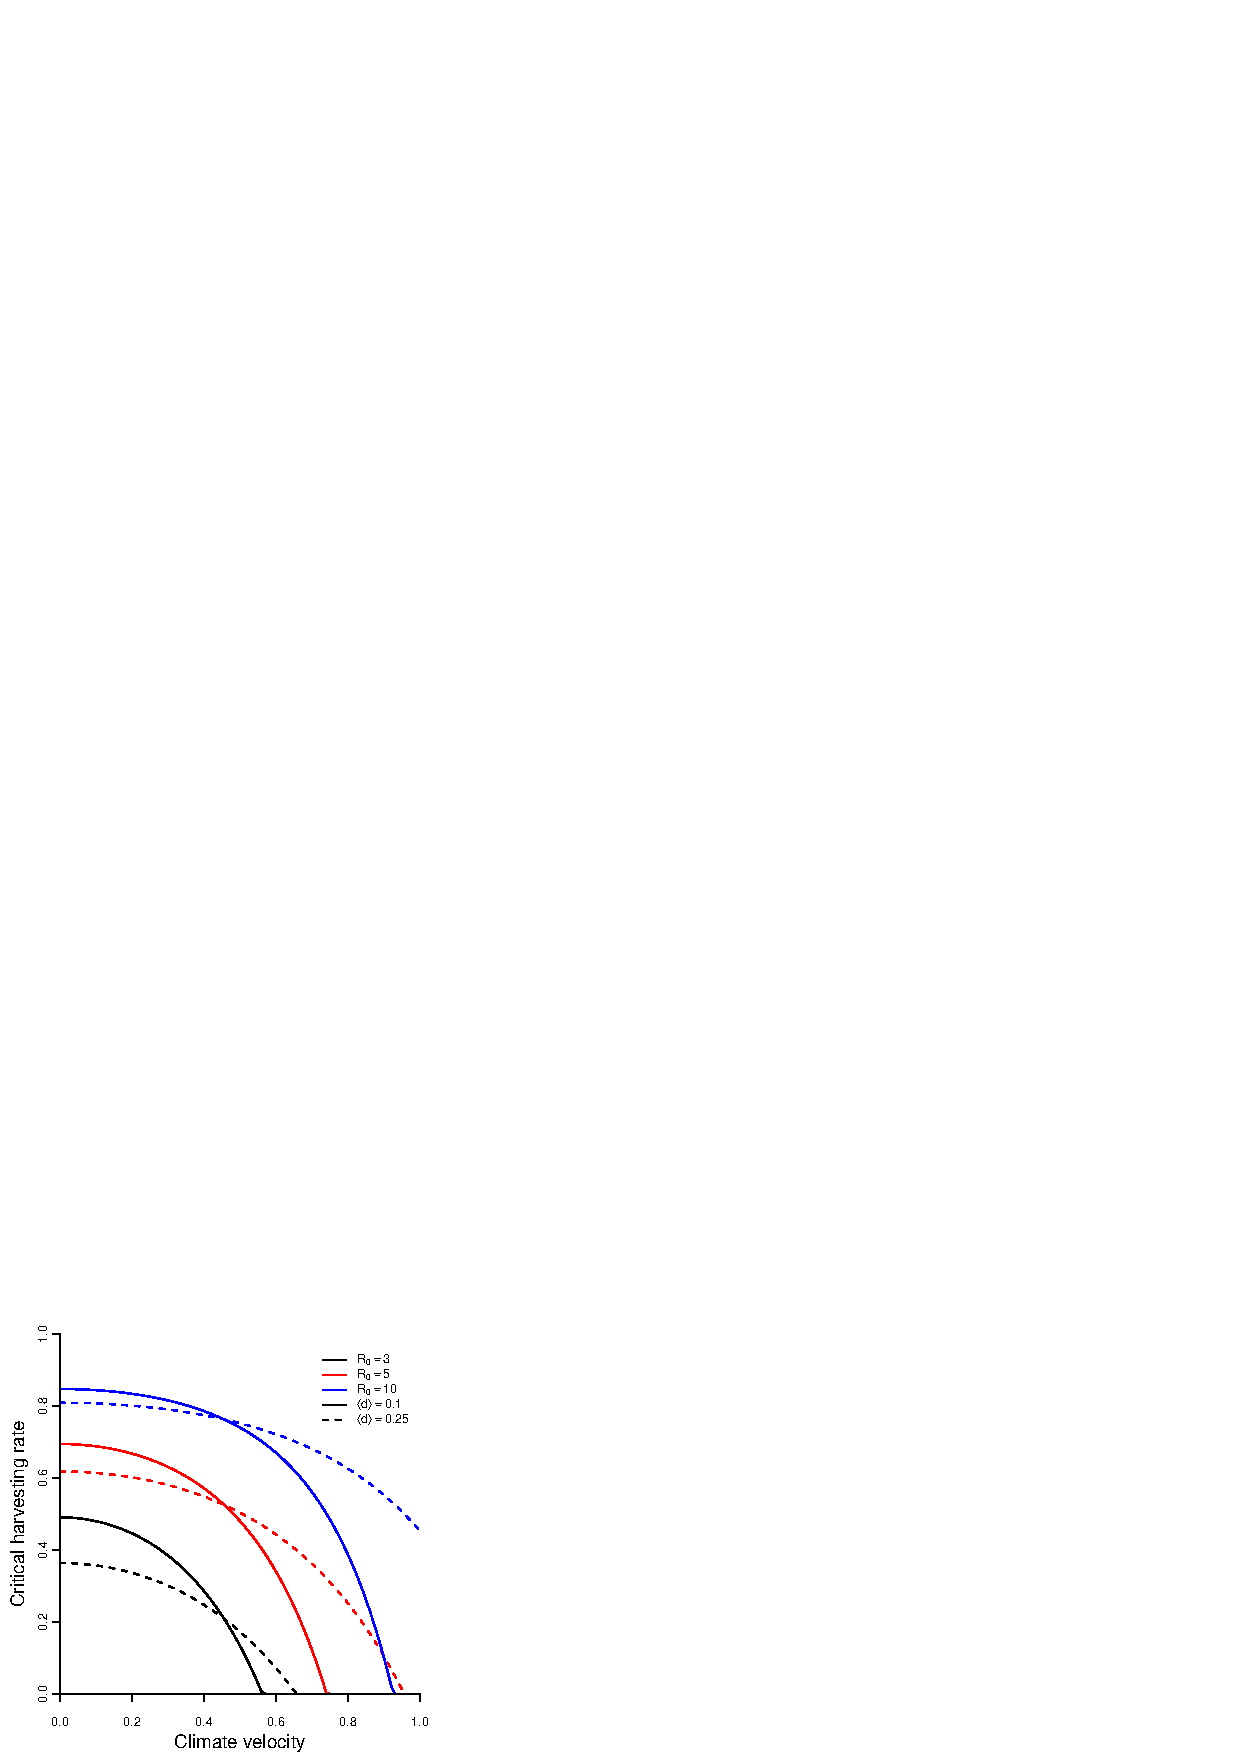
\includegraphics[width=\textwidth]{plots/critical_rates.pdf}
\end{subfigure}
\begin{subfigure}{3in}
\subcaption{\label{biomass}}
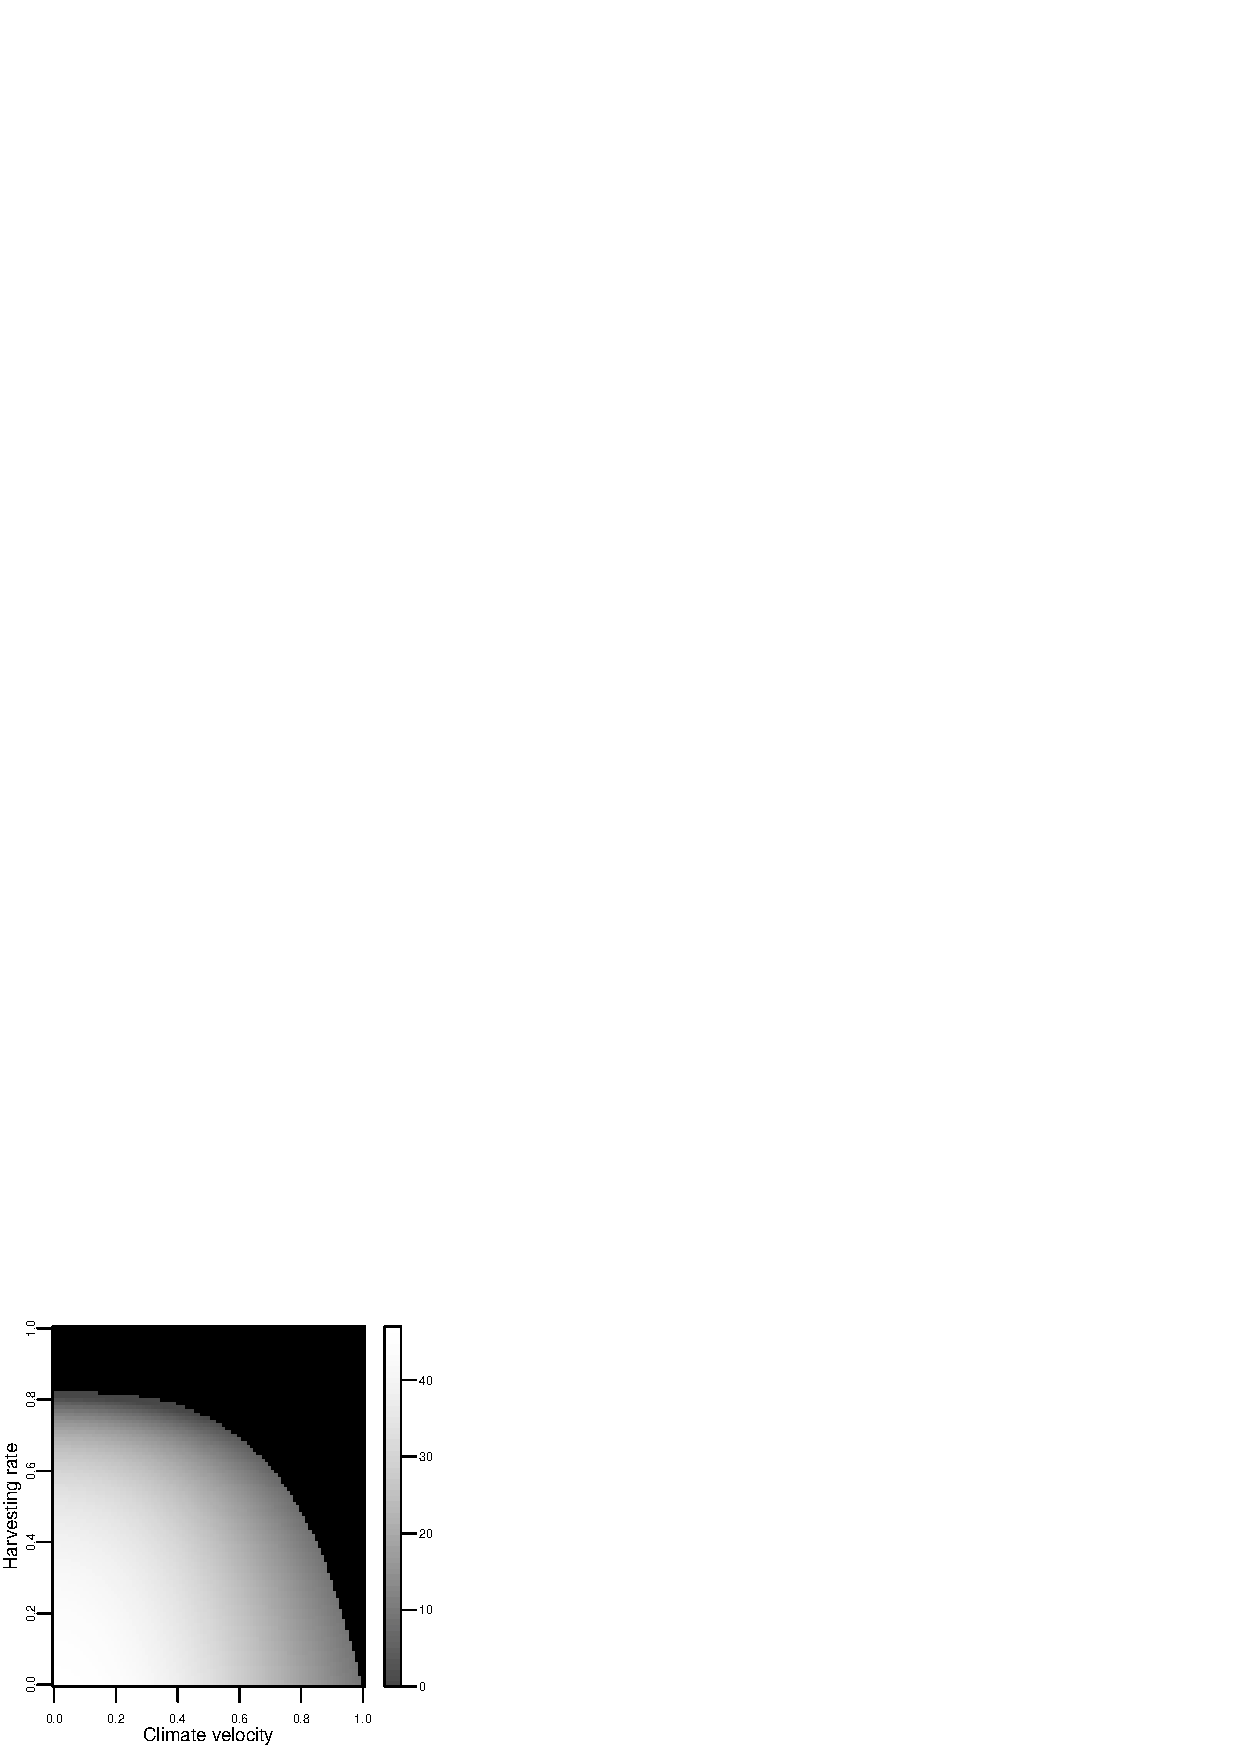
\includegraphics[width=\textwidth]{plots/eqbiomass.pdf}
\end{subfigure}

\caption{%(a) The critical harvesting rate on the y-axis as a function of the rate of environmental shift on the x-axis.  Black lines correspond to a growth rate of $R_0=3$, red to $R_0=7$, and blue to $R_0=10$.  Solid lines correspond to an average dispersal distance $\langle d \rangle =0.1$ and dashed lines correspond to an average dispersal distance $\langle d \rangle =0.25$.  (b) The equilibrium biomass of the population as a function of the rate of environmental shift on the x-axis and the harvesting rate on the y-axis. These results are from a Gaussian dispersal kernel with parameters $L=1$, $R_0=5$, $\langle d \rangle = 0.399$.    These results are from an approximated Gaussian dispersal kernel with $L=1$.
}

\label{baseline}
\end{figure}

\pagebreak

\noindent {\bf Figure \ref{baseline}}: (a) The equilibrium biomass of the population as a function of the rate of environmental shift on the x-axis and the harvesting rate on the y-axis. These results are from a Gaussian dispersal kernel with parameters $L=1$, $R_0=5$, $\langle d \rangle = 0.399$.  (b) The critical harvesting rate on the y-axis as a function of the rate of environmental shift on the x-axis.  Black lines correspond to a growth rate of $R_0=3$, red to $R_0=7$, and blue to $R_0=10$.  Solid lines correspond to an average dispersal distance $\langle d \rangle =0.1$ and dashed lines correspond to an average dispersal distance $\langle d \rangle =0.25$.  These results are from an approximated Gaussian dispersal kernel with $L=1$.

\pagebreak

\begin{figure}[htbp]
\begin{center}
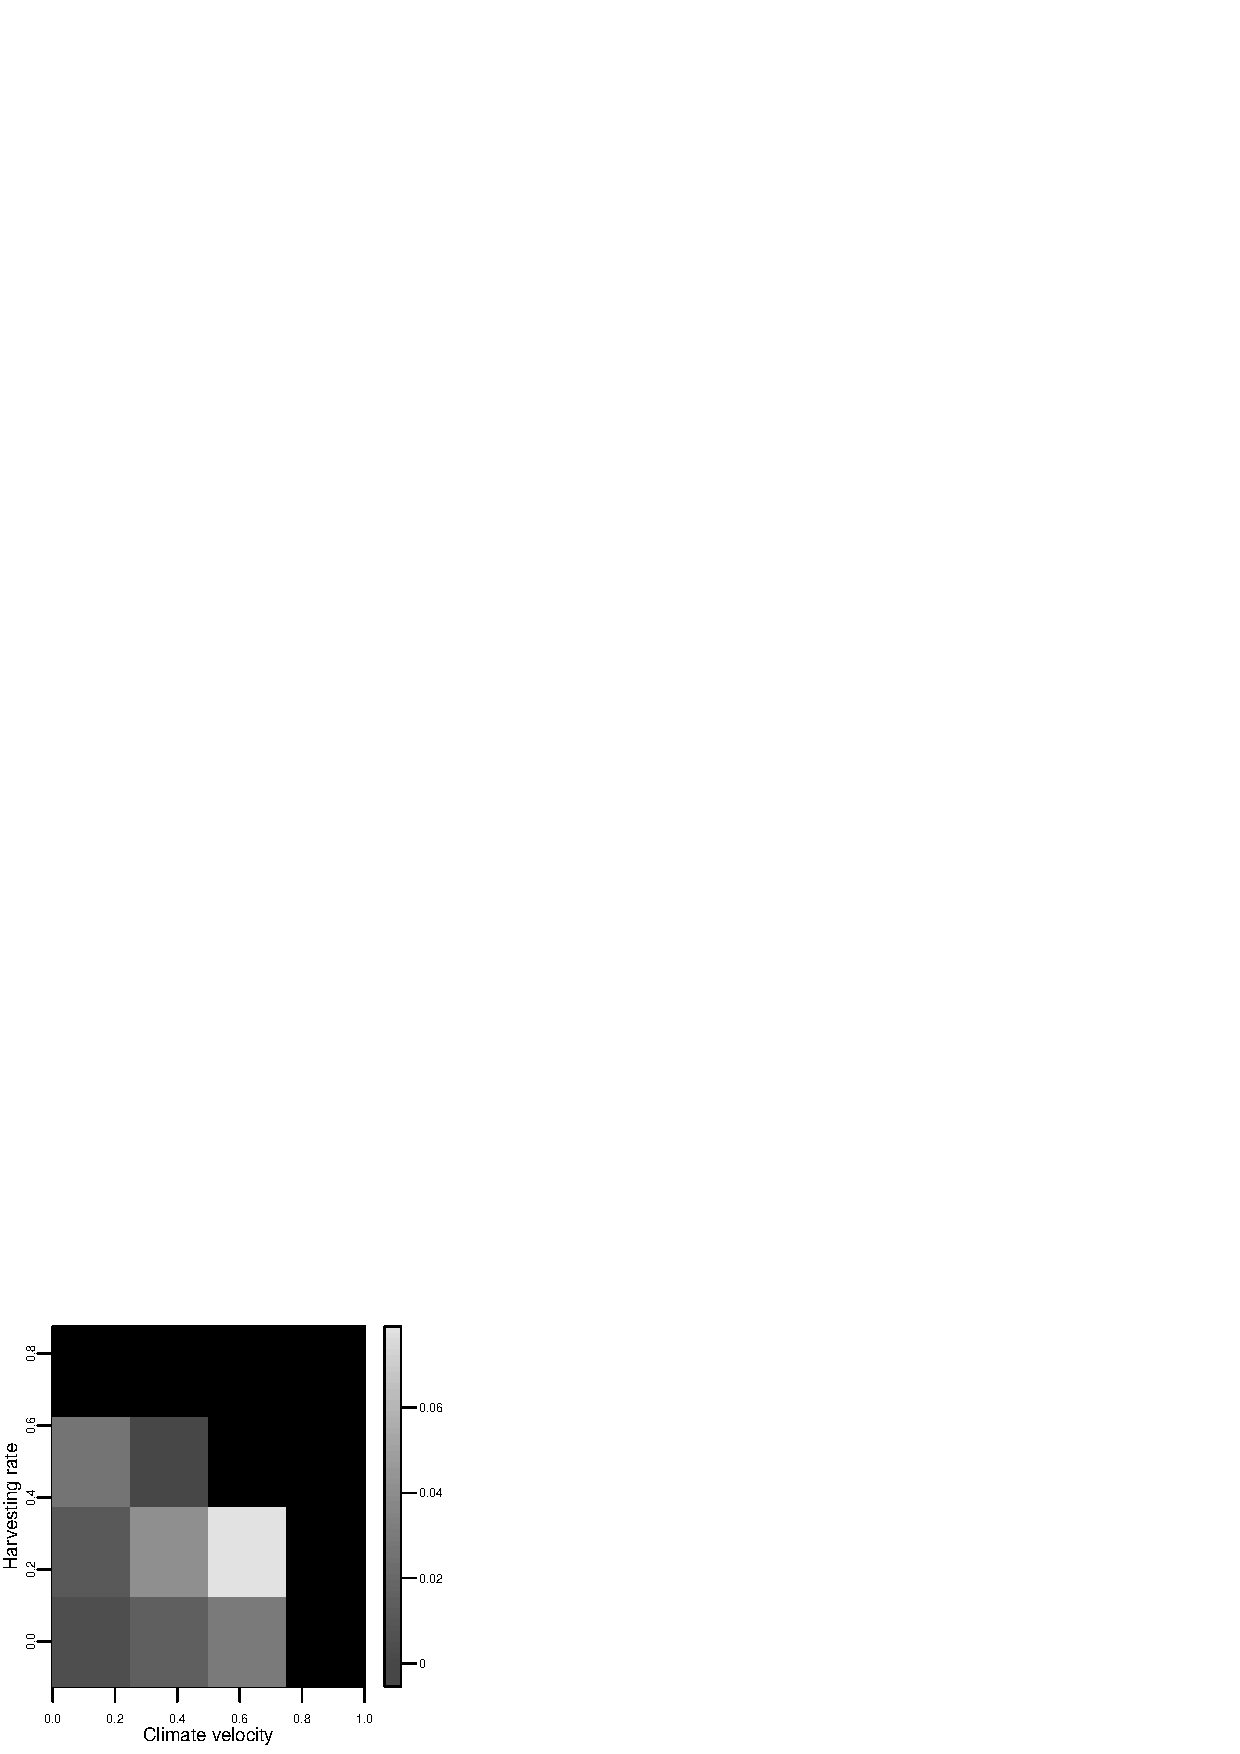
\includegraphics[width=3in]{plots/synergy.pdf}
\caption{
%Positive synergy between the two stressors.  The x-axis shows the rate of environmental shift, the y-axis shows the harvesting rate, and the color indicates the loss in biomass in the doubly stressed population in excess of the sum of the losses caused by each stressor individually, $E_\text{hc}-E_\text{h}-E_\text{c}$.  These results are from an approximated Gaussian dispersal kernel with parameters $L=1$, $R_0=5$, $\langle d \rangle = 0.399$.
}
\label{Synergy}
\end{center}
\end{figure}

\pagebreak

\noindent {\bf Figure \ref{Synergy}}: Positive synergy between the two stressors.  The x-axis shows the rate of environmental shift, the y-axis shows the harvesting rate, and the color indicates the loss in biomass in the doubly stressed population in excess of the sum of the losses caused by each stressor individually, $E_\text{hc}-E_\text{h}-E_\text{c}$.  This excess loss, on the order of $.001$, is small in comparison to the total biomass, which can be as large as $20$.  These results are from an approximated Gaussian dispersal kernel with parameters $L=1$, $R_0=5$, $\langle d \rangle = 0.399$.

\pagebreak

\begin{figure}[htbp]

\begin{subfigure}{.33\textwidth}
\subcaption{}
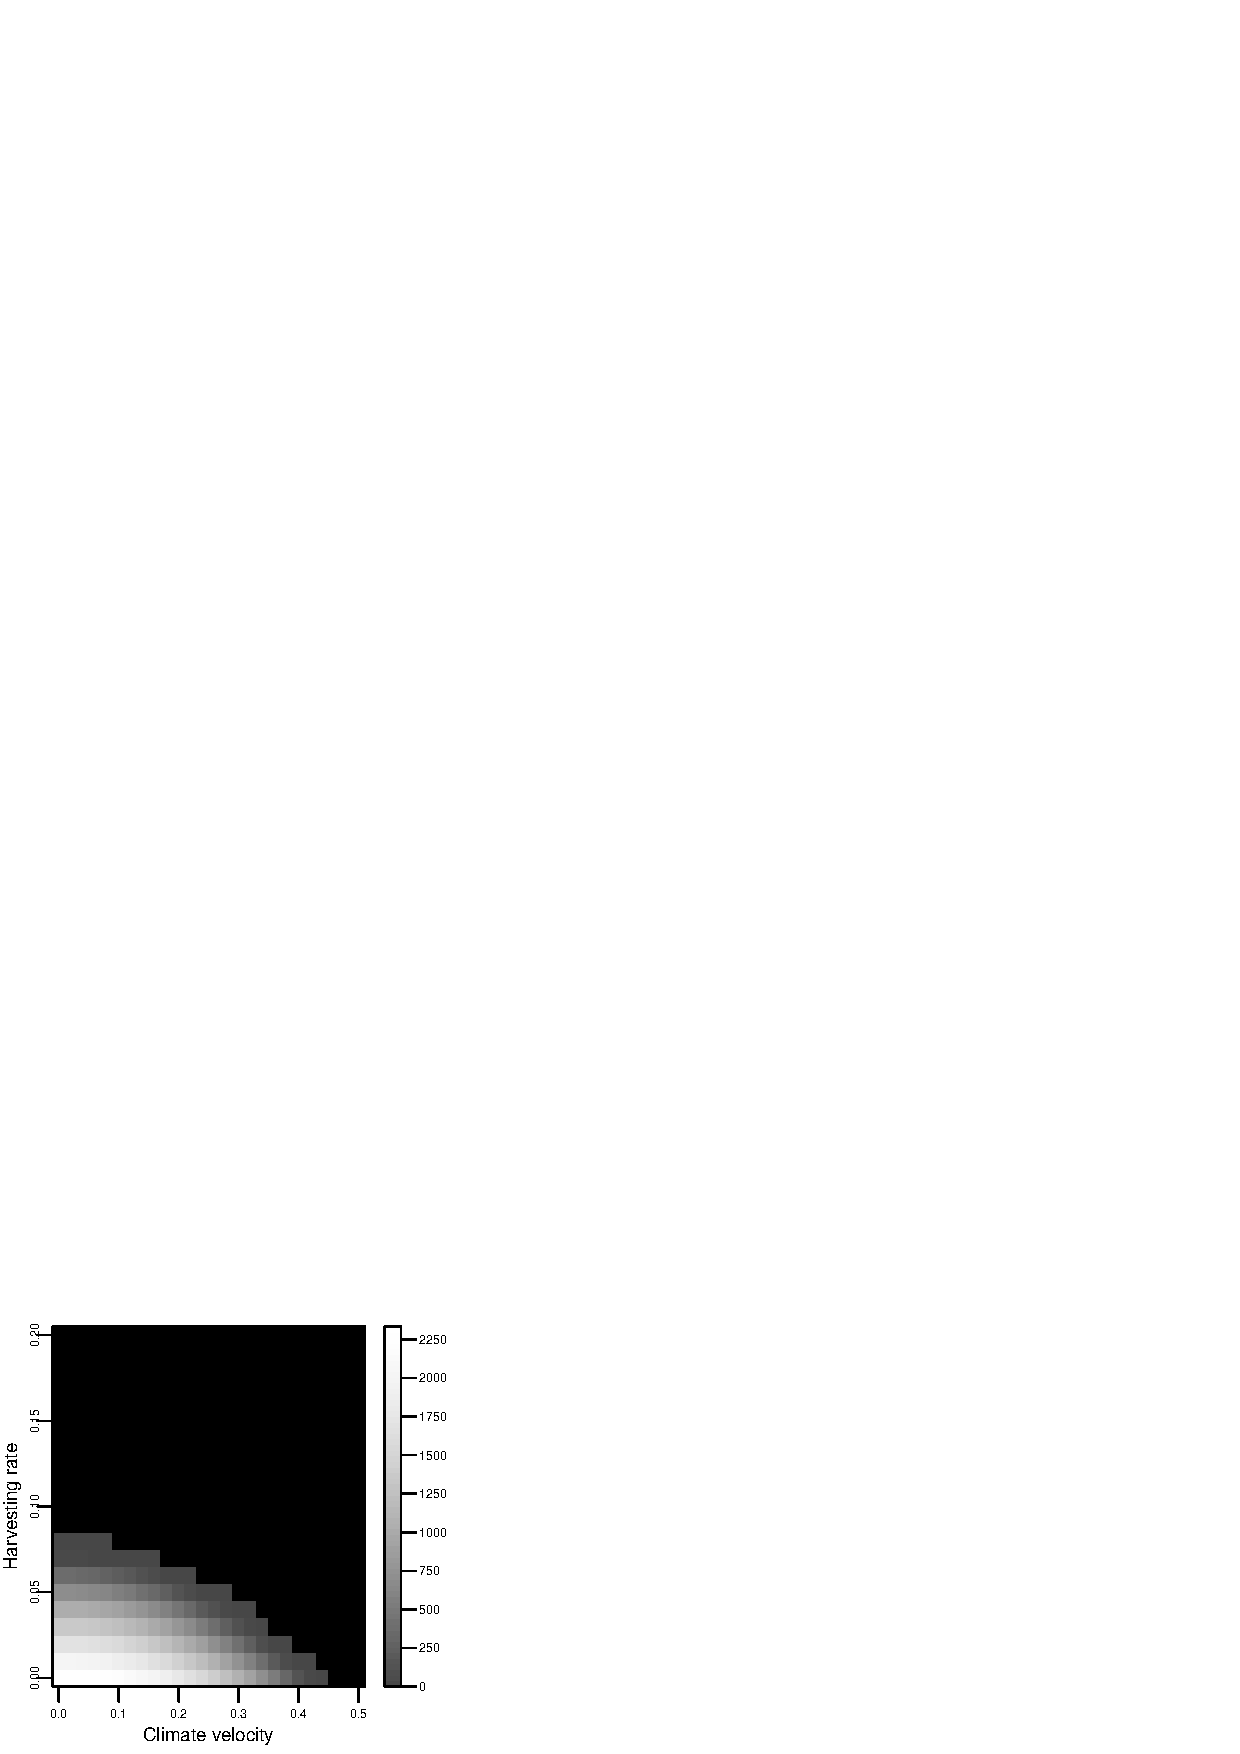
\includegraphics[width=\textwidth]{plots/eqbiomass_sim.pdf}
\label{nomang}
\end{subfigure}
\begin{subfigure}{.33\textwidth}
\subcaption{}
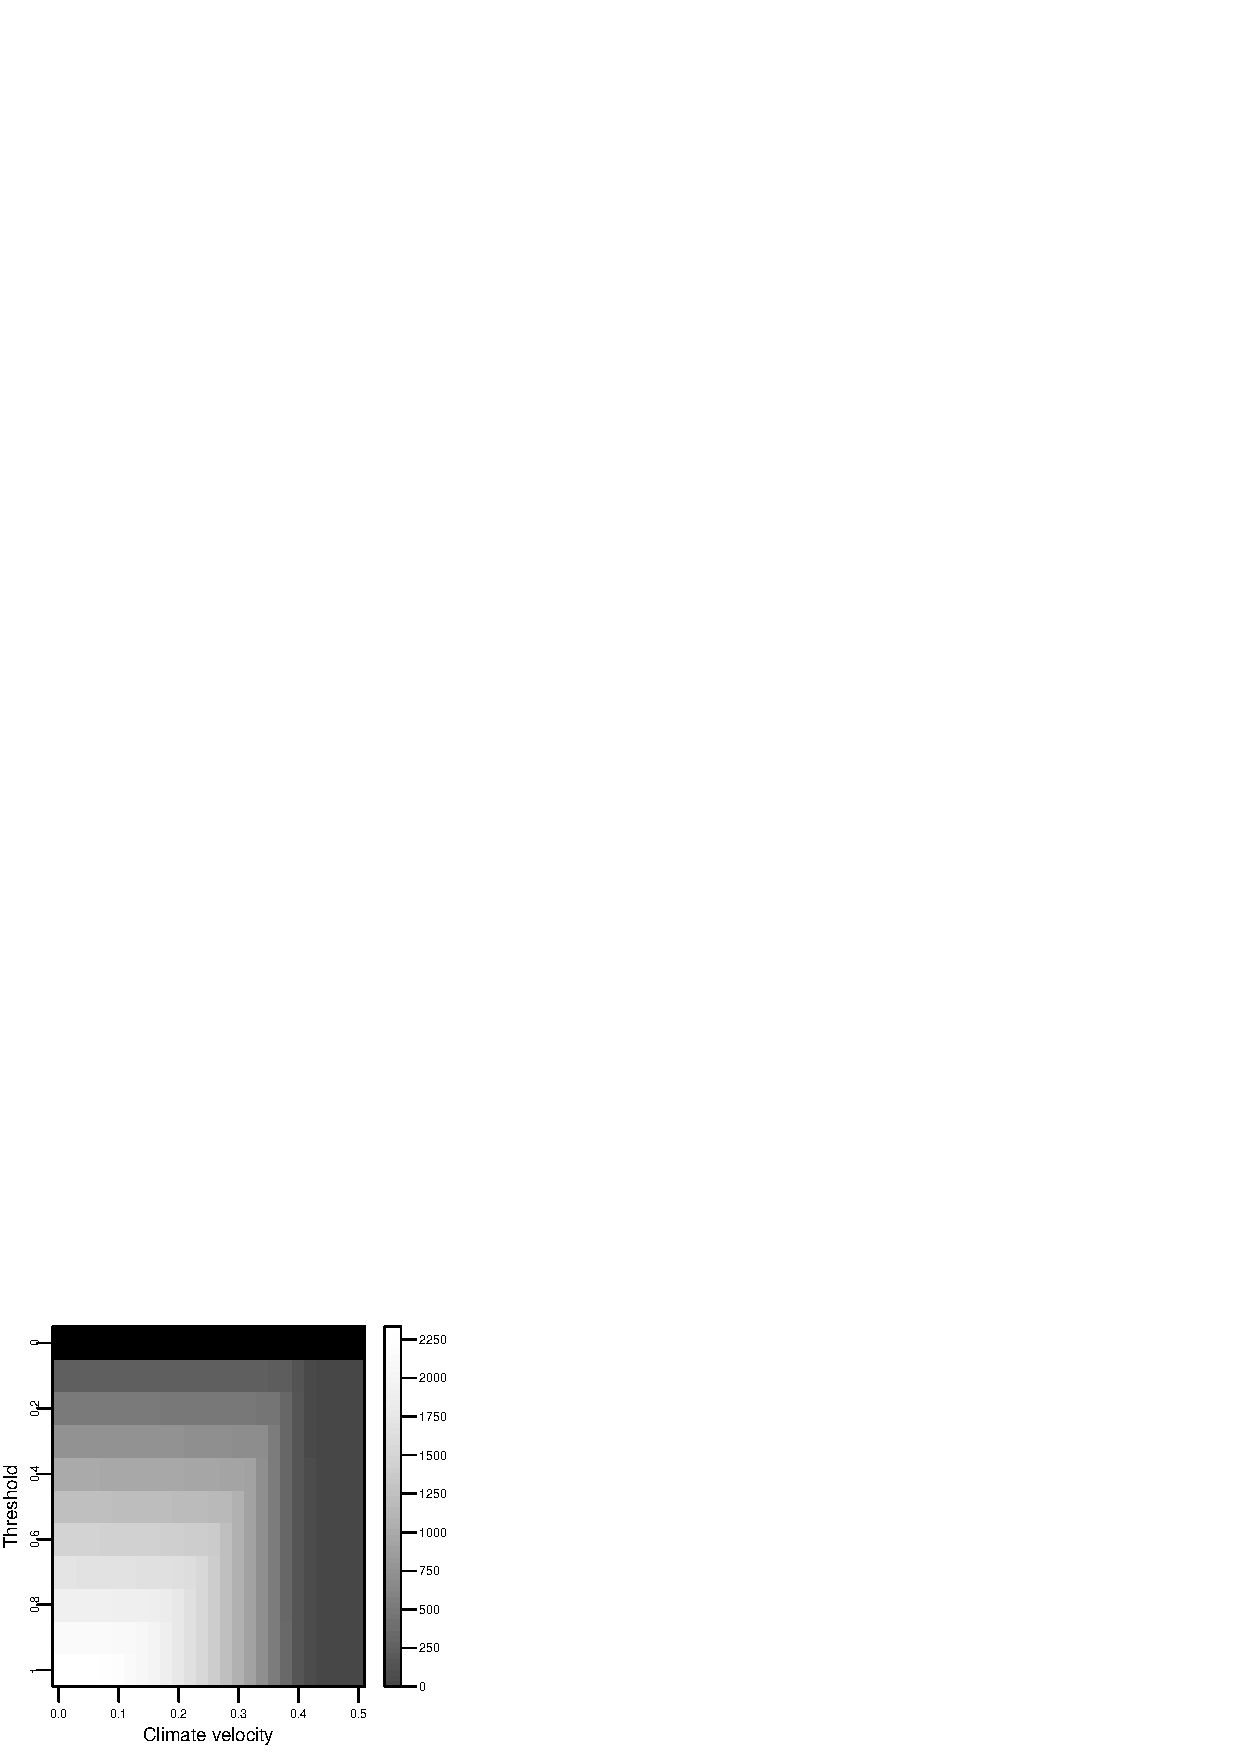
\includegraphics[width=\textwidth]{plots/eqbiomass_thresh.pdf}
\end{subfigure}
\begin{subfigure}{.33\textwidth}
\subcaption{}
\includegraphics[width=\textwidth]{plots/eqbiomass_mpa.pdf}
\end{subfigure}
\caption{
%The equilibrium biomass of the population as a function of the rate of environmental shift on the x-axis and the harvesting rate on the y-axis with and without management strategies.  (a) No management.  (b) Threshold harvesting levels.  (c) MPAs.  These results are from a simulation with a Laplacian dispersal kernel with parameters $L=1$, $R_0=5$, $K=100$, and $\langle d \rangle =2$.
}
\label{management}
\end{figure}

\pagebreak

\noindent {\bf Figure \ref{management}}: The equilibrium biomass of the population as a function of the rate of environmental shift on the x-axis and the harvesting rate on the y-axis with and without management strategies.  (a) No management.  (b) Threshold harvesting levels.  (c) MPAs.  These results are from a simulation with a Laplacian dispersal kernel with parameters $L=1$, $R_0=5$, $K=100$, and $\langle d \rangle =2$.

\pagebreak

\section{Tables}
\begin{table}[h]
\caption{Table of variables used in the text}
\begin{tabular}{@{}lllllll@{}}
  Variable & Definition
\\\cmidrule{1-1} \cmidrule{2-2}   
$n_t(x)$ & density of fish at position $x$ at time $t$
\\ $n^*(\overline{x})$ & density of fish at equilibrium at position $\overline{x}$ relative to the patch 
\\ $k(x-y)$ & dispersal kernel, the probability of larva traveling from position $y$ to position $x$
\\ $\langle d \rangle $ & expected distance traveled by larva
\\ $f(n)$ & recruitment function, the number of offspring produced by a population of size $n$
\\ $R_0$ & intrinsic growth rate, $R_0=f'(0)$
\\ $h$ & proportion of adults harvested
\\ $L$ & patch length
\\ $c$ & rate of environmental shift
\end{tabular}
\label{variables}
\end{table}

\pagebreak

\appendix
\section{Appendix}
In Appendix \ref{stab}, we provide the details for assessing the persistence of a population with an integrodifference model and we discuss the effect of the harvesting function on population persistence.  In Appendix \ref{sep}, we provide the details for assessing population persistence with separable dispersal kernels.  In Appendix \ref{gausapp} and \ref{sinapp}, we derive expressions for the critical harvesting rate and rate of environmental shift for Gaussian and sinuosoidal dispersal kernels.  In Appendix \ref{approxcrit}, we derive approximate expressions for these critical rates.

\subsection{Determining stability \label{stab}}
As in Zhou et al. \citep{ZhouKot2011}, let $k(x-y)$ be a dispersal kernel, let $f(n)$ be a recruitment function, and let $g(n)$ be the harvesting function describing the number of adults harvested from a population of size $n$.  The integrodifference model describing the population over time is given by 

\begin{equation} n_{t+1}(x)=\int_{-L/2+ct}^{L/2+ct}k(x-y)f(n_t(y)-g(n_t(y)))dy. \label{integro} \end{equation}

To find a traveling pulse, we are only interested in the population density as a function of the location within the patch rather than absolute position, $\overline{x}\equiv x-ct$.

\begin{equation*}
n^*(\overline{x})\equiv n^*(x-ct)=n_t(x).   \label{trav} 
\end{equation*}

The integrodifference equation (\ref{integro}) gives us an expression for $n^*$:

\begin{align}
n^*(\overline{x}-c)&=\int_{-L/2}^{L/2}k(\overline{x}-\overline{y})f(n^*(\overline{y})-g(n^*(\overline{y})))d\overline y \notag
\\ \Rightarrow n^*(\overline{x})&=\int_{-L/2}^{L/2}k(\overline{x}+c-\overline{y})f(n^*(\overline{y})-g(n^*(\overline{y}))d\overline y  \label{pulse}
\end{align}
As long as $f(0)=0$, there is a trivial solution to this problem where $n^*(\overline{x})\equiv 0$ for all $\overline{x}\in[-L/2,L/2]$, i.e. there is a trivial traveling pulse with no fish in it.  If the trivial traveling pulse is unstable, even very small populations will persist or grow and avoid crashing back to the trivial pulse.  To evaluate stability a traveling pulse, we introduce a small perturbation to the traveling pulse $n^*(\overline{x})$ and see if this perturbation grows or shrinks over time:

\begin{align}
n_t(x)&=n^*(\overline{x})+\xi_t(x) \notag
\\ \Rightarrow \xi_{t+1}(x)&=n_{t+1}(x)-n^*(\overline{x}) \notag
\\ \Rightarrow \xi_{t+1}(x)&=\int_{-L/2+ct}^{L/2+ct}k(x-y)\big(f(n_t(y)-g(n_t(y)))-f(n^*(\overline{y})-g(n^*(\overline{y}))\big)dy \text{ using (\ref{pulse})} \notag
\\ \Rightarrow \xi_{t+1}(x)&=\int_{-L/2+ct}^{L/2+ct}k(x-y)(1-g'(n^*(\overline{y})))f'(n^*(\overline{y})-g(n^*(\overline{y}))\xi_t(y)dy \notag
\\& \text{ by linearizing around the traveling pulse} \notag
\\ \Rightarrow \xi_{t+1}(x)&=\int_{-L/2+ct}^{L/2+ct}k(x-y)(1-g'(0))f'(0)\xi_t(y)dy \text{ if $n^*(\overline{x})=0$} \label{perturb}
\end{align}


If we assume $\xi_t(x)=\lambda^tu(x-ct)$ for some $\lambda\in\R$ and $u:[-L/2,L/2]\to\R$, then the perturbation grows in time if and only if $\lambda >1$.  Using Equation (\ref{perturb}), we can rewrite $\xi_t(x)$,
\begin{align*}
\lambda u(x-ct-c)&=(1-g'(0))f'(0)\int_{-L/2+ct}^{L/2+ct}k(x-y)u(y-ct)dy
\\ \\\Rightarrow \lambda u(\overline{x})&=(1-g'(0))f'(0)\int_{-L/2}^{L/2}k(\overline{x}+c-\overline{y})u(\overline{y})dy
\end{align*}

Define the integral operator
$$ \psi_f(u)(x)=(1-g'(0))f'(0)\int_{-L/2}^{L/2}k(x+c-y)u(y)dy. $$
Then the perturbation to the traveling pulse will satisfy 
\begin{equation} \psi_f(u)(x)=\lambda u(x) \label{eigen} \end{equation}
$\lambda$ and $u$ are thus an eigenvalue and eigenvector of the functional operator $\psi_f$.  The trivial traveling pulse is unstable when the dominant eigenvalue of $\psi_f$ is greater than $1$.


The biomass in the equilibrium traveling wave depends on the specific functional form of the harvesting function $g(n)$.  However, the persistence of the population only depends on $g'(0)$ so in this paper, we only considered a proportional harvesting function, i.e. the amount of fish harvested obeyed $g(n)=hn$.  For this function, $g'(0)=h$.  

\subsection{Separable dispersal kernels \label{sep}}
Jentzsch's theorem shows that there is an eigenfunction $u$, provided that the kernel $k$ satisfies some properties \citep{ZhouKot2011}.  Finding the eigenfunctions and eigenvalues is in general a hard problem to solve.  It becomes easier if the kernel $k$ is separable, i.e. there are functions $a_n,b_n$ such that $k(x-y)=\sum_{n=1}^\infty a_n(x)b_n(y)$.  In that case, (\ref{eigen}) becomes
\begin{align}
\lambda u(x)&=f'(0)\sum_{n=1}^\infty\left( a_n(x)\int_{-L/2}^{L/2}b_n(y-c)u(y)dy\right) \notag
\\ \Rightarrow \lambda\int_{-L/2}^{L/2}b_k(x-c)u(x)dx&=f'(0)\sum_{n=1}^{\infty}\left(\int_{-L/2}^{L/2}b_n(x-c)u(x)dx\right)\left(\int_{-L/2}^{L/2}a_n(y)b_k(y-c)dy\right) \notag
\\ \Rightarrow \lambda d_k&=f'(0)\sum_{n=1}^\infty A_{nk}d_n  \label{problem}
\end{align}
where
\begin{equation*}
A_{nk}=\int_{-L/2}^{L/2}a_n(x)b_k(x-c)dx \text{ and } d_k=\int_{-L/2}^{L/2}b_k(x-c)u(x)dx
\end{equation*}
Finding the eigenvalues of (\ref{eigen}) then reduces to finding the eigenvalues of the matrix $(A_{nk})_{n,k=1}^\infty$.

\subsection{Gaussian dispersal kernel \label{gausapp}}
The Gaussian dispersal kernel is given by
$$k(x-y)=\frac{1}{2\sqrt{D\pi}}e^{\frac{-(x-y)^2}{4D}}.$$
As in \citep{Latore:1998fk}, this separable kernel can be written as
$$k(x-y)=\sum_{n=0}^\infty a_n(x)b_n(y)$$
where
$$a_n(x)=b_n(x)=\frac{1}{\sqrt{2n!\sqrt{D\pi}}}e^{-x^2/4D}\left(\frac{x}{\sqrt{2D}}\right)^n.$$

As a first approximation to $k$ we ignore all but the $0^{th}$ terms for $a_n$ and $b_n$ so that Equation (\ref{problem}) becomes
\begin{align*}
\lambda d_0(c)&=(1-h)f'(0)A_{00}(c)d_0(c)
\\ \Rightarrow \lambda&=(1-h)R_0A_{00}(c)
\\\text{ where } A_{00}(c)&=2\sqrt{2}\exp\left(\frac{-c^2}{8D}\right)\left[\text{erf}\left(\frac{L-c}{2\sqrt{2D}}\right)-\text{erf}\left(\frac{-L-c}{2\sqrt{2D}}\right)\right]
\end{align*}
where $\text{erf}$ is the error function.  The critical rate of environmental shift $c^*$ and the critical harvesting rate $h^*$ are those values of $c$ and $h$, respectively, that make $\lambda=1$.

\subsection{Sinusoidal dispersal kernel \label{sinapp}}
A sinusoidal dispersal kernel is given by 
$$k(x-y)=\left\{\begin{array}{ccccc}
\frac{w}{2}\cos(w(x-y)) & , & |x-y|\leq\frac{\pi}{2w}
\\ 0 & , & |x-y|>\frac{\pi}{2w}
\end{array}\right.
$$
where $L$ is the length of the patch and we assume $\frac{\pi}{2w}>L,c<\frac{\pi}{2w}-L$.

In this case, $k(x-y)=\frac{w}{2}\cos(wx)\cos(w(y-c))+\frac{w}{2}\sin(wx)\sin(w(y-c))$ so that $A_{ij}$ and $d_i$ can be found for $i,j=1,2$ and (\ref{problem}) reduces to 
$$\lambda^2-\left(\frac{R_0(1-h)wL}{2}\cos(wc)\right)\lambda+\frac{R_0^2(1-h)^2}{16}\left(w^2L^2-\sin^2(wL)\right)=0.$$

If we solve for $\lambda$,we find
\begin{equation*} \lambda=(1-h)R_0\left[\frac{wL\cos(wc)}{4}+\frac{1}{4}\sqrt{\sin^2(wL)-w^2L^2\sin^2(wc)}\right]. \label{cosine} \end{equation*}


Zhou et al. \citep{ZhouKot2011} solve for the critical speed, $c^*$, at which the population will be driven extinct:
$$c^*=c^*(R_0)=\frac{1}{w}\cos^{-1}\left[\frac{16+R_0^2(1-h)^2(w^2L^2-\sin^2(wL))}{8R_0(1-h)wL}\right].$$
Similarly, we can solve for the critical harvesting rate, $h^*$, at which the population will be driven extinct:
$$
h^*=1-\frac{1}{R_0}\cdot\frac{4wL}{w^2L^2-\sin^2(wL)}\left[\cos(wc)-\sqrt{\cos^2(wc)-1+\frac{\sin^2(wL)}{w^2L^2}}\right] 
$$

\subsection{Approximate critical harvesting proportions \label{approxcrit}}
~\\We will use the following Taylor series to make approximations of the critical harvesting proportions under the two dispersal kernels:
\begin{align*}
\cos(x)&=1-\frac{x^2}{2}
\\ \cos^2(x)&=1-x^2
\\ \sin^2(x)&=x^2-\frac{x^4}{3}
\\ erf(x)&=\frac{2}{\sqrt{\pi}}(x-\frac{x^3}{3})
\\ \exp(x)&=1+x+\frac{x^2}{2}
\end{align*}
For the sinusoidal kernel we found 
\begin{equation}
h^*=1-\frac{1}{R_0}\cdot\frac{4wL}{w^2L^2-\sin^2(wL)}\left[\cos(wc)-\sqrt{\cos^2(wc)-1+\frac{\sin^2(wL)}{w^2L^2}}\right] 
\end{equation} 
Using the Taylor series and the fact that $w=\frac{\sqrt{\frac{\pi^2}{4}-2}}{\sigma}$ where $\sigma^2$ is the variance of the sinusoidal kernel,
\begin{align*}
h^*&\sim 1-\frac{1}{R_0}\cdot\frac{12wL}{w^4L^4}\left[1-\frac{w^2c^2}{2}-\sqrt{1-w^2c^2-\frac{w^2L^2}{3}}\right]
%\\&=1-\frac{1}{R_0}\cdot\frac{12}{w^3L^3}\left[1-\frac{w^2c^2}{2}-\sqrt{1-w^2c^2-\frac{w^2L^2}{3}}\right]
%\\&=1-\frac{1}{R_0}\cdot\frac{12\sigma^3}{L^3(\frac{\pi^2}{4}-2)^{3/2}}\left[1-\frac{(\frac{\pi^2}{4}-2)c^2}{2\sigma^2}-\sqrt{1-\frac{(\frac{\pi^2}{4}-2)c^2}{\sigma^2}-\frac{(\frac{\pi^2}{4}-2)L^2}{3\sigma^2}}\right]
%\\&=1-\frac{1}{R_0}\cdot\frac{6\sigma}{L^3(\frac{\pi^2}{4}-2)^{3/2}}\left[2\sigma^2-(\frac{\pi^2}{4}-2)c^2-\frac{2}{\sqrt{3}}\sigma\sqrt{3\sigma^2-(\frac{\pi^2}{4}-2)3c^2-(\frac{\pi^2}{4}-2)L^2}\right]
%\\&=1-\frac{1}{R_0}\cdot\frac{6\sigma}{L^34(\frac{\pi^2}{4}-2)^{3/2}}\left[8\sigma^2-(\pi^2-8)c^2-\frac{4}{\sqrt{3}}\sigma\sqrt{12\sigma^2-(\pi^2-8)3c^2-(\pi^2-8)L^2}\right]
%\\&=1-\frac{12}{R_0L^3(\pi^2-8)^{3/2}}\cdot\sigma\left[8\sigma^2-(\pi^2-8)c^2-\frac{4}{\sqrt{3}}\sigma\sqrt{12\sigma^2-(\pi^2-8)3c^2-(\pi^2-8)L^2}\right]
\\&=1-\frac{1}{R_0}\cdot\frac{4\sqrt{3}}{L^3(\pi^2-8)^{3/2}}\cdot\sigma\left[8\sqrt{3}\sigma^2-(\pi^2-8)\sqrt{3}c^2-4\sigma\sqrt{12\sigma^2-(\pi^2-8)(3c^2+L^2)}\right]
\end{align*}
For the Gaussian kernel we found 
\begin{equation}
h^*=1-\frac{2\sqrt{2}\exp\left(\frac{c^{2}}{8D}\right)}{R_0\left[erf\left(\frac{L-c}{2\sqrt{2D}}\right)-erf\left(\frac{-L-c}{2\sqrt{2D}}\right)\right]}
\end{equation} 
Using the Taylor series and the fact that $D=\frac{\sigma^2}{2}$ where $\sigma^2$ is the variance of the exponential kernel,
\begin{align*}
h^*&\sim 1-\frac{\sqrt{2\pi}(1+\frac{c^2}{8D}+\frac{c^4}{128D^2})}{R_0\sqrt{\pi}\left[\frac{L-c}{2\sqrt{2D}}-\frac{(L-c)^3}{3(2\sqrt{2D})^3}-\frac{-L-c}{2\sqrt{2D}}+\frac{(-L-c)^3}{3(2\sqrt{2D})^3)}\right]}
%\\&= 1-\frac{\sqrt{2\pi}(1+\frac{c^2}{8D}+\frac{c^4}{128D^2})}{R_0\left[\frac{2L}{2\sqrt{2D}}+\frac{-L^3+3L^2c-3Lc^2+c^3-L^3-3L^2c-3Lc^2-c^3}{3(2\sqrt{2D})^3}\right]}
%\\&= 1-\frac{\sqrt{2\pi}(1+\frac{c^2}{8D}+\frac{c^4}{128D^2})}{R_0\left[\frac{L}{\sqrt{2D}}-2\frac{L^3+3Lc^2}{3(2\sqrt{2D})^3}\right]}
%\\&= 1-\frac{\sqrt{2\pi}(1+\frac{c^2}{8D}+\frac{c^4}{128D^2})}{R_0L\left[\frac{48D-2(L^2+3c^2)}{3(2\sqrt{2D})^3}\right]}
%\\&= 1-\frac{3*32D\sqrt{D\pi}(1+\frac{c^2}{8D}+\frac{c^4}{128D^2})}{R_0L\left(48D-2(L^2+3c^2)\right)}
%\\&= 1-\frac{3*32D\sqrt{D\pi}(\frac{128D^2+16c^2D+c^4}{128D^2})}{R_0L\left(48D-2(L^2+3c^2)\right)}
%\\&= 1-\frac{3\sqrt{\pi}(128D^2+16c^2D+c^4)}{4R_0L\sqrt{D}\left(48D-2(L^2+3c^2)\right)}
%\\&= 1-\frac{3\sqrt{2\pi}(32\sigma^4+8c^2\sigma^2+c^4)}{4R_0L\sigma\left(24\sigma^2-2(L^2+3c^2)\right)}
\\&= 1-\frac{1}{R_0}\cdot\frac{3\sqrt{2\pi}}{8L}\frac{(32\sigma^4+8c^2\sigma^2+c^4)}{\sigma\left(12\sigma^2-(L^2+3c^2)\right)}
\end{align*}
In the case of both kernels, the critical harvesting proportion can be approximated by a function that looks like 
\begin{equation}
h^*\sim1- \frac{1}{R_0}\cdot C(L)f(\sigma^2,c^2,L^2+3c^2)
\end{equation}
where $C(L,R_0)$ is a decreasing function of the length of the viable patch and the intrinsic growth rate.

\end{document}
